\section{Where the limit lies in software terms}\label{sec:software}

So far the software reference has been ``a 31-node ESN with input noise $3\times10^{-3}$ under realistic noise''. The convention refers
the laser intensity noise to the input through the modulation depth (Section~\ref{sec:tasks}), but it strongly affects the conclusion:
in Table~\ref{tab:encodings} the mask ties with the ESN on Mackey--Glass ($3.3\times10^{-4}$ against $3.2\times10^{-4}$), whereas with
input noise $10^{-3}$ the ESN reaches $5.3\times10^{-5}$, about 6 times better than the mask and about 3 times better than the best
single ring with the readout-side changes. This section therefore does not use a single point: it sweeps the software input noise
from 0 to $3\times10^{-3}$ and places the resonator on that curve, answering ``how large and how noisy a software reservoir is one
resonator equivalent to''.

\subsection{Sweeping the software input noise}

Figure~\ref{fig:software} shows the test error of 31-, 100- and 300-node ESNs (and of NG-RC~\cite{gauthier2021} for the closed-loop
task) against input noise, with the same protocol as the resonator (Section~\ref{sec:protocol}); the best resonators of the previous
sections are drawn as horizontal reference lines. The top axis converts input noise to the effective number of bits (ENOB) of an
analog-to-digital converter (ADC): if the full scale spans the input range, $N$-bit quantization noise has an rms of $2^{-N}/\sqrt{12}$, so $10^{-4}$,
$3\times10^{-4}$, $10^{-3}$ and $3\times10^{-3}$ correspond to about 11.5, 9.9, 8.2 and 6.6 bits.

\begin{figure}[htbp]
\centering
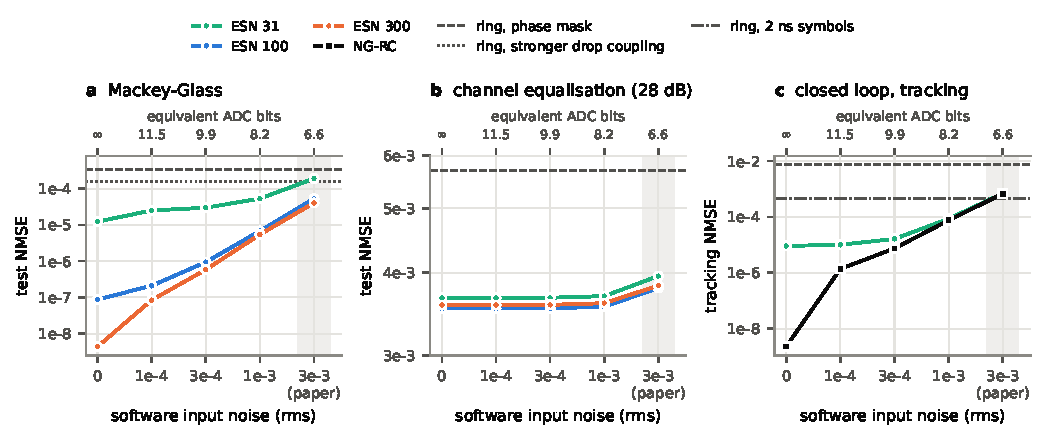
\includegraphics[width=\linewidth]{figS3_esn_input_noise}
\caption{Test error of software reservoirs against their input noise (rms); the top axis gives the equivalent ADC effective bits $N$
(noise $2^{-N}/\sqrt{12}$). Curves: ESNs with 31, 100 and 300 nodes, and NG-RC (closed loop only); horizontal lines: resonators under
realistic noise (plain spectral-phase mask, stronger drop coupling, $2~\mathrm{ns}$ symbols). The grey band marks the convention
$3\times10^{-3}$ used in the previous sections.
(a) Mackey--Glass; (b) channel equalisation (SNR $28~\mathrm{dB}$); (c) closed-loop tracking of a commanded trajectory of the Hénon
map (Appendix~\ref{app:closedloop}). Same selection and re-test protocol as the resonator; Mackey--Glass is the geometric mean over
three series, channel equalisation uses a single series except at $3\times10^{-3}$, and the closed loop averages four training
records.}
\label{fig:software}
\end{figure}

\emph{Mackey--Glass.} The 31-node ESN reaches $1.2\times10^{-5}$, $2.5\times10^{-5}$, $3.0\times10^{-5}$, $5.3\times10^{-5}$ and
$1.9\times10^{-4}$ at input noise 0, $10^{-4}$, $3\times10^{-4}$, $10^{-3}$ and $3\times10^{-3}$; 100- and 300-node ESNs reach
$5.3\times10^{-5}$ and $4.0\times10^{-5}$ at $3\times10^{-3}$, and $8.8\times10^{-8}$ and $4.4\times10^{-9}$ without noise. The best
single ring ($1.55\times10^{-4}$) crosses the 31-node ESN at an input noise of about $2.5\times10^{-3}$; the 100- and 300-node ESNs are
better over the whole sweep, 3 to 4 times at $3\times10^{-3}$.

\emph{Channel equalisation, fibre link and NARMA-10.} The error of the first two tasks comes mostly from the channel's own noise:
lowering the 31-node ESN's input noise from $3\times10^{-3}$ to 0 only moves its error from $3.95\times10^{-3}$ to
$3.66\times10^{-3}$, and growing the ESN to 300 nodes barely matters, but over the whole sweep they beat the best resonator
($5.7\times10^{-3}$); on the fibre link the ESN reaches $1.8\times10^{-2}$ and the best resonator $2.0\times10^{-2}$
(Appendix~\ref{app:fibre}). On NARMA-10 even at $3\times10^{-3}$ the 31-, 100- and 300-node ESNs reach $0.11$, $0.041$ and $0.032$,
better than the single ring's $0.19$.

\emph{Closed-loop decisions.} Appendix~\ref{app:closedloop} uses the resonator to predict the next step of the Hénon map and applies a
bounded control based on the prediction. When tracking a commanded trajectory, the resonator with $2~\mathrm{ns}$ symbols reaches a
tracking error of $4.5\times10^{-4}$ (mean over four training records; $4.4\times10^{-4}$ for the first record shown in
Appendix~\ref{app:closedloop}); the error of the software predictors is set entirely by their input noise and crosses the
resonator at about $2.4\times10^{-3}$, and at $10^{-3}$ the 31-node ESN and NG-RC reach $8.6\times10^{-5}$ and $7.5\times10^{-5}$,
about 5 times better. A second closed-loop task, holding the unstable fixed point of the Hénon map (Appendix~\ref{app:closedloop}), needs only linear
feedback, so the software's modelling capacity is not the limit there, which makes it the cleanest calibration: its crossing is at
about $1.7\times10^{-3}$ (not shown in Fig.~\ref{fig:software}).

The three directly comparable tasks (Mackey--Glass, trajectory tracking and holding the fixed point; on channel equalisation the
curves do not cross) agree: the best single ring matches a 31-node ESN with input noise of about $1.7\times10^{-3}$ to
$2.5\times10^{-3}$, i.e.\ by the conversion above an ADC with about \emph{7 effective bits} (6.9 to 7.4). The ESN curves are medians of
three random reservoirs, and the reservoir-to-reservoir spread (a factor of about 1.7 at $3\times10^{-3}$) moves these crossings by
roughly half a bit. The conversion assumes that the full scale spans the input range $[0,1]$; ENOB as specified for converters refers
to a full-scale sine wave, which differs from this by a fraction of a bit.

\subsection{What 7 bits mean}

This number must be read at the rate at which the resonator works. Our resonator needs $Q\sim10^{6}$ for enough Kerr nonlinearity,
i.e.\ symbol rates of about $0.5$ to $1~\mathrm{GBd}$. Converter resolution falls with sampling rate~\cite{walden1999}; at these rates
off-the-shelf converters offer about 9 effective bits (for
example, a 12-bit converter sampling at $3.2~\mathrm{GSa/s}$ is specified at about 9 effective bits~\cite{ti_adc12dj3200}); converters
with 5 to 6 effective bits are acquisition systems at above $100~\mathrm{GSa/s}$ with tens of gigahertz of bandwidth (for example about
5.9 bits at $33~\mathrm{GHz}$ and 5.0 bits at $110~\mathrm{GHz}$ bandwidth~\cite{keysight_uxr}), and at those rates the resonator's $Q$
can only be $2\times10^{4}$ to $4\times10^{4}$, where the Kerr effect is nearly unused (in the fibre-link task of
Appendix~\ref{app:fibre}, a resonator operated at $28~\mathrm{GBd}$ is only about 15\% better than a linear equaliser). In other
words, at the rates where the resonator works, digitising the signal and handing it to a 31-node software reservoir is no less
accurate than the resonator; a resonator can only be needed where the signal is optical to begin with and digitisation is the very
step to be avoided.

\subsection{The readout must be quantized too}\label{sec:quant}

The software input noise was interpreted above as ADC quantization noise, but the resonator's 31 readings must also be digitised,
and none of the previous results included this step. To make the comparison symmetric we attach one $N$-bit converter to each reading
of the best single ring (Table~\ref{tab:quant}). The full scale of each channel is calibrated once on the run used for fitting and
kept for the test run, i.e.\ the gain is calibrated and then fixed. We consider two front ends: a linear converter digitising the
photocurrent, and a logarithmic amplifier before the converter (equal relative steps, matching the logarithm of the readout). The
reference is a 31-node ESN whose input is quantized to $N$ bits with no other noise, i.e.\ the software side gets a real quantizer
instead of equivalent Gaussian noise.

% generated by experiments/make_table3.py; do not edit by hand
\begin{table}[htbp]
\centering
\caption{Readout quantization. Each of the 31 readings of the best single ring (stronger drop coupling, realistic noise, Mackey--Glass) has its own $N$-bit converter, with the full scale of each channel calibrated once on the fitting run and kept for the test run; ``linear'' digitises the photocurrent, ``log'' places a logarithmic amplifier before the converter. Reference: a 31-node ESN (one random reservoir) whose input is quantized to $N$ bits, with no other noise. Geometric mean over three series $\times$ six new pairs. Unquantized, the resonator reaches $1.5\times10^{-4}$ and the noise-free ESN $2.4\times10^{-5}$.}
\label{tab:quant}
\small
\begin{tabular}{cccc}
\toprule
bits $N$ & resonator, linear & resonator, log amplifier & ESN 31, quantized input \\
\midrule
4 & $4.2\times10^{-3}$ & $1.9\times10^{-3}$ & $3.5\times10^{-3}$ \\
5 & $2.2\times10^{-3}$ & $1.1\times10^{-3}$ & $1.3\times10^{-3}$ \\
6 & $1.2\times10^{-3}$ & $5.6\times10^{-4}$ & $4.5\times10^{-4}$ \\
7 & $6.0\times10^{-4}$ & $3.5\times10^{-4}$ & $2.3\times10^{-4}$ \\
8 & $3.6\times10^{-4}$ & $2.7\times10^{-4}$ & $1.3\times10^{-4}$ \\
9 & $2.7\times10^{-4}$ & $2.1\times10^{-4}$ & $9.3\times10^{-5}$ \\
10 & $2.0\times10^{-4}$ & $1.8\times10^{-4}$ & $6.8\times10^{-5}$ \\
12 & $1.6\times10^{-4}$ & $1.6\times10^{-4}$ & $4.6\times10^{-5}$ \\
\bottomrule
\end{tabular}
\end{table}


The resonator needs many bits not to be degraded by quantization: both front ends need 10 bits to come within 1.3 times of the
unquantized error ($1.54\times10^{-4}$); at 7 bits they reach $6.0\times10^{-4}$ and $3.5\times10^{-4}$, 2 to 4 times worse. The
line powers span several orders of magnitude, so a linear converter gives weak lines few steps; the logarithmic amplifier helps but
does not remove this. At every depth from 6 to 12 bits the ESN with an input quantized to the same depth is 1.2 to 3.4 times better
than the resonator with all 31 channels quantized (against the logarithmic front end; more against the linear one); only at very
coarse quantization, 4 and 5 bits, is the resonator with a logarithmic amplifier better than the ESN, and there both errors are above
$10^{-3}$. Read the other way, the unquantized resonator ($1.54\times10^{-4}$) lies between the ESN with 7- and 8-bit input
quantization ($2.3\times10^{-4}$ and $1.3\times10^{-4}$), consistent with the roughly 7 bits from the equivalent-noise conversion.

Including the readout quantization therefore only makes the comparison less favourable for the resonator: software needs one
converter at its input, the resonator 31, each with about 10 effective bits. Such converters exist at $1~\mathrm{GBd}$, but the power
and cost of 31 channels are a real price. Weighting in the optical domain (computing the readout's linear combination with a spectral
shaper and balanced detection) would need a single converter, but then the delay taps must be implemented with optical delay lines;
we did not simulate such a readout.

\subsection{The limit of ring arrays}

About half of a single ring's error comes from its own detuning jitter and shot noise (Section~\ref{sec:noise}), which are independent
between rings. When several rings with different masks share one input comb and their readouts are concatenated (31 lines $\times$ 8
taps per ring), this part averages out. With 16 times the training length (16\,320 symbols), 1, 2, 4, 8, 16 and 32 rings with stronger
drop coupling reach $1.27\times10^{-4}$, $3.4\times10^{-5}$, $1.36\times10^{-5}$, $8.4\times10^{-6}$, $6.7\times10^{-6}$ and
$6.9\times10^{-6}$: no further gain beyond 16 rings, i.e.\ the error saturates at about 1/19 of a single ring. Letting all rings share
the same laser intensity noise (one input comb split among all rings) barely changes this ($6.8\times10^{-6}$ for 16 rings), so the
saturation does not come from common-mode source noise. With the same training length, ESNs with 100, 300 and 1000 nodes and input noise
$3\times10^{-3}$ reach $3.9\times10^{-5}$, $2.1\times10^{-5}$ and $1.4\times10^{-5}$, so 16 rings are 2 to 6 times better; but with input
noise $10^{-3}$ (one series) they reach $6.8\times10^{-6}$, $3.2\times10^{-6}$ and $1.65\times10^{-6}$: a 100-node ESN already ties with
16 rings and a 1000-node ESN is about 4 times better. An array thus only moves the limit somewhat along the software axis without
changing the conclusion. More rings help only when the task is limited by the rings' own noise: on channel equalisation at
$28~\mathrm{dB}$ channel SNR neither more rings nor a larger ESN helps.

\subsection{Why the $3\times10^{-3}$ convention is strict}

$3\times10^{-3}$ is the laser intensity noise ($10^{-3}$) divided by the modulation depth ($0.33$), which assumes that the software's
input is as noisy as the resonator's. But this source hardly affects the resonator: with only the laser intensity noise on
(Section~\ref{sec:breakdown}) the resonator's error rises only 1.5 to 1.9 times, while the 31-node ESN's error already doubles at input
noise $10^{-4}$. The same intensity noise hurts the resonator far less than it hurts the ESN once referred to the input (possibly
because in the resonator it acts on the pump and all input lines at once and partly appears as a common-mode change; we did not test
this separately). The convention $3\times10^{-3}$ is therefore strict on software, and the statements ``on par with the 31-node ESN''
in the previous sections hold under this strict convention; a fairer point is around $10^{-3}$, where software is better on every task
in this paper.

The conclusion of this section: \emph{within the design space explored and on the tasks studied, the accuracy of a Kerr-microcomb
reservoir stays below that of a software reservoir of the same size; the best single resonator found matches a 31-node ESN fed through
a converter with about 7 effective bits}. This is a statement about one device class (a $200~\mathrm{GHz}$ silica resonator), one
readout (31 drop-port lines, logarithm, linear ridge regression) and one noise model, not a bound for all microcomb reservoirs. The
evaluation protocol is part of it: a single noise realisation is optimistic by 10 to 30\%, results in the chaotic regime are not
reproducible, and the input noise given to software reverses the comparison, so we give whole curves rather than one point.
Section~\ref{sec:bidir} raises the resonator by about one bit with a second set of modes and an optimised mask, against software that
is optimised in the same way.
